Systematic uncertainties that affect the sensitivity of our di-Higgs search
come from a variety of sources such as theoretical uncertainties on
cross sections or proton structure, experimental uncertainties related
to the modelling of the detector response, the amount of collected
data, and the discrepancies between the simulated samples and the real data.

Systematic uncertainties can be divided into two broad categories:
those affecting only the yields of selected events from different processes
(the "normalization" uncertainties) and those that, in addition to the change in rate, may
distort the shape of the \mTHH distribution used in the extraction of
the limits (the "shape" uncertainties). %Systematic uncertainties of all types enter the likelihood function of the fit in the limits extraction as independent nuisance parameters.                                                                                                                                                                                                                                                                                                                                                                                                                                                                                                                                                                     

\subsection{Normalization uncertainties}

%Normalization uncertainty for each source of the systematic bias is determined through variation of parameters governing the impact of that bias and measuring the effect of such variation on the yield of signal and background components of the sample. The size of the effect then enters the likelihood fit as a constraint on the corresponding nuisance parameters.                                                                                                                                                                                                                                                                                                                                                                             

The sources of systematic
uncertainties that affect normalizations are discussed in the list below. The sizes of some
systematic uncertainties may vary depending on the resonance mass hypothesis
and the decay channel of the leptonically decaying \PZ boson, in which cases
ranges of the uncertainty values are listed. Normalization uncertainties
discussed in this section do not affect the normalizations of the \ttbar and DY
backgrounds because those are determined from data during the simultaneous fit of the signal and control regions.

\begin{itemize}

\item{\bfseries Luminosity} - CMS estimated this uncertainty on the integrated
  luminosity of the CMS 2016 data set to be $2.5\%$
  ~\cite{CMS-PAS-LUM-17-001}. This uncertainty directly affects the
  expected event yields for the signal processes as well as all
  background processes except for the two dominant backgrounds, DY and
  \ttbar. %, which have their normalization determined in the limits extraction likelihood fit.

\item{\bfseries Pileup} - Signal and background event yields depend on the
  accuracy of the reproduction of pileup interactions in each simulated event. The effect of pileup is considered on each process. The recommended nominal value of 69.2 mb is used for the total inelastic pp cross section, for Down and Up variations, the values of 66.02 and 72.38 mb are used respectively, reflecting the imperfect knowledge of the total inelastic
  proton-proton interaction cross section at 13~TeV. The effect is seen only in the normalization and we, thus, consider this a normalization uncertainty and assign the value of $6\%$.

\item{\bfseries Proton PDF} - The systematic bias associated with the limited
  knowledge of the interacting proton content is evaluated using an ensemble of a hundred of PDF
  replicas from the NNPDF set \cite{Ball:2014uwa} following the
  PDF4LHC prescription \cite{Botje:2011sn,Alekhin:2011sk} and the RMS
  of the resulting process normalizations is taken as a measure of the
  bias. It is found to be of order 5\%.

\item{\bfseries QCD scales} - Theoretical uncertainties in the QCD
  factorization and renormalization scales affect the expected yield
  of the signal and background events, excluding the \ttbar and DY
  yields as mentioned earlier. This uncertainty is estimated
  by varying independently these two scales in simulation by factors 0.5 and 2 with respect to the nominal
  values of the scales. The unphysical cases with one of the scales
  fluctuating up while the other fluctuates down are discarded. In
  each bin of the HH transverse mass distribution the maximum and
  minimum variation are used to build an envelope around the nominal
  shape, resulting in the effect of the size 4-6\% on the processes' yields.

%\item{\bfseries Theoretical cross sections} - The theoretical cross section is  used to normalize the contribution from the single top  background. The uncertainty in this cross section is propagated to  the uncertainty in the background yields for this process and is   found to be 5--7\%.

% \item {\bfseries MET}: the effect of the JEC and JER on the MET is studied modifying MET variables that go into HH transverse mass shape used in the final fit. The effect of the calibration of unclustered MET, meaning missing energy associated with particles that are not clustered into jets, is found only on the normalization, the shape itself is not distorted. The size of the effect is $~3\%$ depending on the mass hypothesis and the $3\%$ normalization uncertainty is used in the analysis.
%

\item{\bfseries Missing transverse energy/momentum} - Clustered energy in
  jets and leptons undergo energy corrections during event
  reconstruction, however, neutral hadrons and photons that do not belong to any jet
  ("unclustered energy") and jets with low transverse momenta (below
  10~GeV) lack such corrections. This results in a small systematic
  bias in the reconstructed missing transverse momentum. \ETslash enters the \mTHH variable, thus the effect of the unclustered energy has to be studied. We shift the energy of each
  particle not contained in jets or contained in low-\pt jets by its
  uncertainty Up and Down. Such variations affect the event yields of signal and background processes at about
  3\% level but do not have a visible effect on the shape of the HH
  transverse mass, thus this source is categorised as a
  "normalization" systematic source.

\end{itemize}



\subsection{Shape uncertainties}

Several sources of systematic uncertainties affect not only the rate but also the shapes of various
kinematic distributions which are inputs to the BDT or a part of the \mTHH construction, the BDT discriminant itself, and the shape of the \mTHH distribution. Each source is varied separately within one standard deviation up and down, and
the effect is propagated through all related variables resulting in
the nominal shape of the HH invariant mass distribution and two
modified shapes corresponding to the Up and Down variations. Such triplet of shapes is prepared for each channel, each mass hypothesis, and for all processes. %both for the signal and control regions of the kinematic phase space.                                                                                                                                                                                                                                                                                                                                                                                                                                                                                                                                                                                       

All these shapes are fit simultaneously in the
signal extraction likelihood fit. The discussion of the these sources
of uncertainties follows.



\begin{itemize}

\item{\bfseries Lepton efficiency} - The effect of the detector on the reconstruction of the lepton: identification and isolation selection
  criteria, and the requirement to pass trigger selection requirements are studied separately and are used to account for data/MC discrepancies. The corrections are derived
  from large dedicated samples of \PZ boson decays and also have an error associated with the procedure. 
  %are themselves known with limited accuracy. 
  The uncertainty on lepton efficiency corrections are derived
  as a function of lepton $p_T$ and $\eta$ and is propagated to the final \mTHH distributions.
  The effect of these uncertainties is sub-percent for the muon
  channel and up to 6\% for the electron channel.


\item{\bfseries Jet energy scale} - The uncertainty on the jet energy scale
  affects \HBB mass and \pt, which are inputs to the BDT. In addition, jet energy scale directly affects \HBB mass and \ETslash, which are used during the construction of the HH invariant mass. %Several factors affecting the calibration of the jet energy scale are considered independently as they are uncorrelated. 
  Jet energy scale is varied Up and Down within one standard deviation of its uncertainty %for each of these factors 
  as a function of jet $p_T$ and $\eta$, and the
  effect on the jet kinematics and on the \ETslash is calculated and
  propagated through the steps of the measurement yielding the
  variation of the HH invariant mass shape.  Jet energy scale
  uncertainty, with all factors combined, has the effect on the yields
  of the signal and some background components as large as 5 to 10\%.

\item{\bfseries Jet energy resolution} - Data and MC a different energy
  resolution, which also affects the final \mTHH shapes via its effect on the dijet invariant
  mass for \HBB and its effect on the \ETslash. Jet energy resolution
  is varied in simulation by one standard deviation as a function of
  jet $p_T$ and $\eta$ and the effect is propagated through the steps
  of the measurement. Its effect on the \mTHH yield is typically order of 0.5\%.

\item{\bfseries b-tagging and mistagging} - The efficiency to tag a \Pqb-jet and the
  probability to misidentify a different flavor or a gluon jet and tag it as a
  \Pqb-jet is corrected in MC samples by factors derived from
  flavor-enhanced jet samples. The uncertainties on these corrections
  are propagated through the whole analysis setup. The effect of the
  \Pqb-tagging efficiency (mistagging/flavor misidentification) is about 5\% (7--10\%) for the Drell-Yan process and at the sub-percent level for other processes (7--10\%).
% to  about 5\% for the Drell-Yan process, while the flavor misidentification impact is larger and is seen to be in the range 7--10\% for most processes.                                                                                                                                                                                                                                                                                                                                                                                                                                                                                                                                                                                                

\item{\bfseries Bin-by-bin uncertainties} - Since the available statistics for the simulated MC samples is limited, the lack of events in some bins of the \mTHH distribution is addressed by bin-by-bin (BBB) uncertainty. This effect may result in sizeable fluctuations of the bin content of the HH invariant mass shapes that enter the
  likelihood fit. Therefore, for each bin of the HH invariant mass distributions
  an individual nuisance parameter is added to the likelihood fit with the Gaussian constraint of one standard deviation of
  the yield uncertainty in that bin.
  
\end{itemize}







%\begin{sidewaystable}
%\begin{center}
%\caption{Yield variations, ee channel, 300 GeV.}
%\begin{tabular}{ | c | c | c | c | c | c |c | c | } \hline
% sample & b-tagging &  mistag &  electron IDnISO &  electron tracker &  electron trigger &  jet resolution &  jet scale \\\hline
%  DY &              4.3 &     7.4 &              5.4 &               1.1 &               2.1 &             0.2 &        5.3 \\
%  TT &              0.5 &     7.4 &              4.7 &               1.1 &               1.9 &             0.0 &        0.5 \\
%  signal\_bbzz &    0.2 &     7.6 &              5.0 &               1.1 &               2.0 &             0.7 &        5.8 \\
%  signal\_bbww &    0.0 &     7.6 &              6.7 &               1.1 &               2.9 &             0.0 &        1.6 \\\hline
%\end{tabular}
%\label{normalization_electron}
%\end{center}
%%---------------------------------------------------------------------                                        
%%Vertical lines as column separators                                                                          
%\begin{center}
%\caption{Yield variations, mm channel, 300 GeV.}
%\begin{tabular}{ | c | c | c | c| c | c | c | c| c |}\hline
%sample &  b-tagging &  mistag &  muon ID &  muon ISO &  muon tracker &  muon trigger &  jet resolution &  jet scale \\\hline
%  DY &              4.9 &     7.0 &      0.2 &       0.1 &           0.1 &           0.4 &             0.2 &        9.4 \\
%  TT &              0.9 &     7.2 &      0.2 &       0.1 &           0.0 &           0.4 &             0.6 &        0.7 \\
%  signal\_bbzz &    0.3 &     7.7 &      0.2 &       0.1 &           0.0 &           0.4 &             0.5 &        4.4 \\
%  signal\_bbww &    0.0 &     9.2 &      0.2 &       0.1 &           0.0 &           0.1 &             0.0 &        8.5 \\\hline
%\end{tabular}
%\label{yieldVariations}
%\end{center}
%%\end{table}
%\end{sidewaystable}
%\begin{sidewaystable}
%\begin{center}
%\caption{Yield variations, ee channel, 300 GeV.}
%\begin{tabular}{ | c | c | c | c | c | c |c | c | } \hline
% sample & b-tagging &  mistag &  electron IDnISO &  electron tracker &  electron trigger &  jet resolution &  jet scale \\\hline
%  DY &              4.3 &     7.4 &              5.4 &               1.1 &               2.1 &             0.2 &        5.3 \\
%  TT &              0.5 &     7.4 &              4.7 &               1.1 &               1.9 &             0.0 &        0.5 \\
%  signal\_bbzz &    0.2 &     7.6 &              5.0 &               1.1 &               2.0 &             0.7 &        5.8 \\
%  signal\_bbww &    0.0 &     7.6 &              6.7 &               1.1 &               2.9 &             0.0 &        1.6 \\\hline
%\end{tabular}
%\label{normalization_electron}
%\end{center}
%%---------------------------------------------------------------------                                        
%%Vertical lines as column separators                                                                          
%\begin{center}
%\caption{Yield variations, mm channel, 300 GeV.}
%\begin{tabular}{ | c | c | c | c| c | c | c | c| c |}\hline
%sample &  b-tagging &  mistag &  muon ID &  muon ISO &  muon tracker &  muon trigger &  jet resolution &  jet scale \\\hline
%  DY &              4.9 &     7.0 &      0.2 &       0.1 &           0.1 &           0.4 &             0.2 &        9.4 \\
%  TT &              0.9 &     7.2 &      0.2 &       0.1 &           0.0 &           0.4 &             0.6 &        0.7 \\
%  signal\_bbzz &    0.3 &     7.7 &      0.2 &       0.1 &           0.0 &           0.4 &             0.5 &        4.4 \\
%  signal\_bbww &    0.0 &     9.2 &      0.2 &       0.1 &           0.0 &           0.1 &             0.0 &        8.5 \\\hline
%\end{tabular}
%\label{yieldVariations}
%\end{center}
%%\end{table}
%\end{sidewaystable}
%\begin{sidewaystable}
%\begin{center}
%\caption{Yield variations, ee channel, 300 GeV.}
%\begin{tabular}{ | c | c | c | c | c | c |c | c | } \hline
% sample & b-tagging &  mistag &  electron IDnISO &  electron tracker &  electron trigger &  jet resolution &  jet scale \\\hline
%  DY &              4.3 &     7.4 &              5.4 &               1.1 &               2.1 &             0.2 &        5.3 \\
%  TT &              0.5 &     7.4 &              4.7 &               1.1 &               1.9 &             0.0 &        0.5 \\
%  signal\_bbzz &    0.2 &     7.6 &              5.0 &               1.1 &               2.0 &             0.7 &        5.8 \\
%  signal\_bbww &    0.0 &     7.6 &              6.7 &               1.1 &               2.9 &             0.0 &        1.6 \\\hline
%\end{tabular}
%\label{normalization_electron}
%\end{center}
%%---------------------------------------------------------------------                                        
%%Vertical lines as column separators                                                                          
%\begin{center}
%\caption{Yield variations, mm channel, 300 GeV.}
%\begin{tabular}{ | c | c | c | c| c | c | c | c| c |}\hline
%sample &  b-tagging &  mistag &  muon ID &  muon ISO &  muon tracker &  muon trigger &  jet resolution &  jet scale \\\hline
%  DY &              4.9 &     7.0 &      0.2 &       0.1 &           0.1 &           0.4 &             0.2 &        9.4 \\
%  TT &              0.9 &     7.2 &      0.2 &       0.1 &           0.0 &           0.4 &             0.6 &        0.7 \\
%  signal\_bbzz &    0.3 &     7.7 &      0.2 &       0.1 &           0.0 &           0.4 &             0.5 &        4.4 \\
%  signal\_bbww &    0.0 &     9.2 &      0.2 &       0.1 &           0.0 &           0.1 &             0.0 &        8.5 \\\hline
%\end{tabular}
%\label{yieldVariations}
%\end{center}
%%\end{table}
%\end{sidewaystable}













%
%
%Systematic uncertainties may change the derived limits. Uncertainties
%that we consider may change the normalization or distort the shape
%that we used for fits. The following sources of the uncertainties have
%been included:
%\begin{itemize}
%
% \item {\bfseries Luminosity}: an uncertainty of $2.5\%$ is assigned for
%   2016 luminosity. All the processes are affected except those, which normalization is determined using data driven methods: DY and \ttbar normalization
%
% \item {\bfseries Lepton Efficiency}: identification, isolation, tracker,
%   and trigger scale factors have been determined using the standard EGamma POG and Muon POG technique of the Tag-and-Probe. 
%   Up and Down variations with respect to the nominal value of the scale factor (within the uncertainty on the value) have been propagated to the final HH transverse mass shape that goes to the fit with the Higgs Combination Tool. Each scale factor type (identification, isolation, tracker,
%   and trigger scale factor) is propagated independently. Overall, the effect of the lepton efficiency, when dealing with b jets, is a very minor
%   one.  These uncertainties are included in both electron and muon channels.
%
% \item {\bfseries MET}: the effect of the JEC and JER on the MET is studied modifying MET variables that go into HH transverse mass shape used in the final fit. The effect of the calibration of unclustered MET, meaning missing energy associated with particles that are not clustered into jets, is found only on the normalization, the shape itself is not distorted. The size of the effect is $~3\%$ depending on the mass hypothesis and the $3\%$ normalization uncertainty is used in the analysis.
%
% \item {\bfseries Jet Energy Scale}: following JetMET group recommendation we check the effect of this uncertainty
%   on all jet-related variables that enter BDT and/or HH system. The scale value is varied Up and Down and modified HH
%   transverse mass shapes are obtained and used in the final fit.
%
% \item {\bfseries Jet Energy Resolution}: we vary up and down jet energy
%   resolution by one $\sigma$ and modify all the jet related
%   variables that are a part of the BDT and/or HH system prior to constructing the final shape. Varied HH transverse mass shapes are used in the final fit.
%
% \item {\bfseries B-jet Tagging and mistag uncertainties}: following the suggestions from the BTV POG
%   b tag and mistag scale factors are applied to all MC samples. The effect of the usage of 
%   light and heavy flavor scale factors is propagated to the final shapes.
%
% %% \item {\bfseries PDF uncertainties}: impossibility to know precisely the
% %%   content of the colliding proton or gluon is addressed in this
% %%   uncertainty. Using the recommended values from LHC Higgs Cross Section group documented in the CERNYellowReportPageAt13TeV we assign $O(1-5)\%$ uncertainties to quark-quark initiated
% %%   processes and $O(10-20)\%$ uncertainties to gluon-gluon uncertainties depending on the process.
%  
% %% \item {\bfseries QCD scale variations}: The uncertainty on the QCD normalization scale for each
% %%   individual process is assigned to a corresponding specific theory error suggested by CMS generator group, which maintains a twiki page with a collection of cross sections for Standard Model processes to be used in the CMS analyses. More information on how the cross-sections and the associated theory errors have been determined is available at ~\cite{SMxsec}. 
%
%\item {\bfseries QCD scale variations}: This uncertainty is estimated by varying the renormalization ($\mu_{R}$) and the factorization ($\mu_{F}$) scales, independently by a factor of 2, meaning from the nominal value of 1 to values of 0.5 and 2. Unphysical situations with one scale fluctuating up and the other fluctuating down are not considered. In each bin of the distribution the maximum (minimum) variation is used as an estimate of the QCD scale uncertainties for all the background and signal samples. The resulting effect has been found on the normalization at the order of $4-6\%$.
%
%
%\item {\bfseries PDF uncertainties}: impossibility to know precisely the
%   content of the colliding proton or gluon is addressed in this
%   uncertainty. The RMS of each of the 101 NNPDF MC variations of the strong coupling constant for each simulated background and signal processes is calculated and the largest one is assigned as a normalization uncertainty, and is of the order of $5\%$. 
%
%
%
%
%
%%% \item {\bfseries PDF uncertainties}: impossibility to know precisely the
%%%    content of the colliding proton or gluon is addressed in this
%%%    uncertainty. For each process, the RMS of each of the 101 NNPDF MC variations is calculated and the largest one is assigned as a normalization un\
%%% certainty, and is of the order of $5\%$.
%
%%%  \item {\bfseries QCD scale variations}: The QCD scale normalization and factorization at $1/2$ and 2 have been applied to each sample and the resulting e\
%%% ffect has been found to be $4-6\%$.
%
%
%
%
%
% %\item {\bfseries Cross section normalization}: Uncertainty associated with the cross section value for the
%   %\ttbar and single top processes. We used the same numbers as in bbVV analysis.
%
% \item {\bfseries Pile up }: The effect of pile up on each
%   process is considered. The recommended nominal value of 69.2 mb is used for the total inelastic pp cross section, for Down and Up variations, the values of 66.02 and 72.38 mb are used respectively. The effect is seen only in the normalization and we, thus, switch to the normalization uncertainty and assign the value of $6\%$.
%
%
% \item {\bfseries Drell-Yan and \ttbar normalizations }: \ttbar and Drell-Yan
%   normalizations we extract from the simultaneous fit of both signal
%   region and DY and \ttbar ~control regions. Normalizations of main backgrounds are allowed to float freely to let the fitter find the best values of the DY and \ttbar normalizations to fit the existing data. HH transverse mass distributions are used in the fit. Separately, an option of control regions only fit has been studied and results were found consistent with the DY and \ttbar normalizations obtained from the fit where signal region was included. Overall, the normalization of \ttbar is near the value
%   '1', deviating up to $\approx10-20\%$ depending on the mass point. DY normalization is deviating higher from the value of '1' since the requirement on 2 b jets and a high boost pushes DY process to higher pT and flavor phase space that is not well modeled in the MC. Therefore, a part of the analysis strategy was to extract these numbers using the real data. The final $\chi^2$ values after the application of \ttbar and Drell-Yan normalizations are near the value '1'.
%
% \item {\bfseries Bin-by-bin uncertainties } To account for the low statistics in some bins of HH transverse mass distribution in MC, bin-by-bin uncertainties should be used. If the error on the MC in the bin is zero, the bin is skipped entirely. However, if the error is non zero and if the number of effective events for each given process is lower than or equal to zero, a Poisson-constrained parameter will be created. Otherwise a Gaussian-constrained parameter is assigned to this bin. Barlow-Beeston algorithm is used to create these bin-by-bin parameters which scale the total yield in the bin. The advantage of this algorithm is that each nuisance parameter has a simple analytic form and analytic minimization can be performed, which results in the reduction of the fit time and an increase of the fit stability.
%
% \item {\bfseries Shape uncertainties}: All shape systematic
%   uncertainties are addressed separately and all together are used in the final fit. The following uncertainties are considered as shape
%   uncertainties: each of lepton scale factors, b tag scale factors of
%   both light and heavy flavour, effect of JEC and JER on all the variables used in
%   BDT and/or HH system. For all these shape uncertainties we
%   propagate the source of uncertainty through all the related
%   variables that enter our BDT or region selection all the way to
%   building the HH candidate and obtaining the final shape.  We
%   produce, therefore, final shapes with the 'nominal value' as well
%   as with 1~$\sigma$ 'Up' and 'Down' variations. 
%
%\end{itemize}


%% \begin{center}
%% \begin{figure}[tbp]
%% %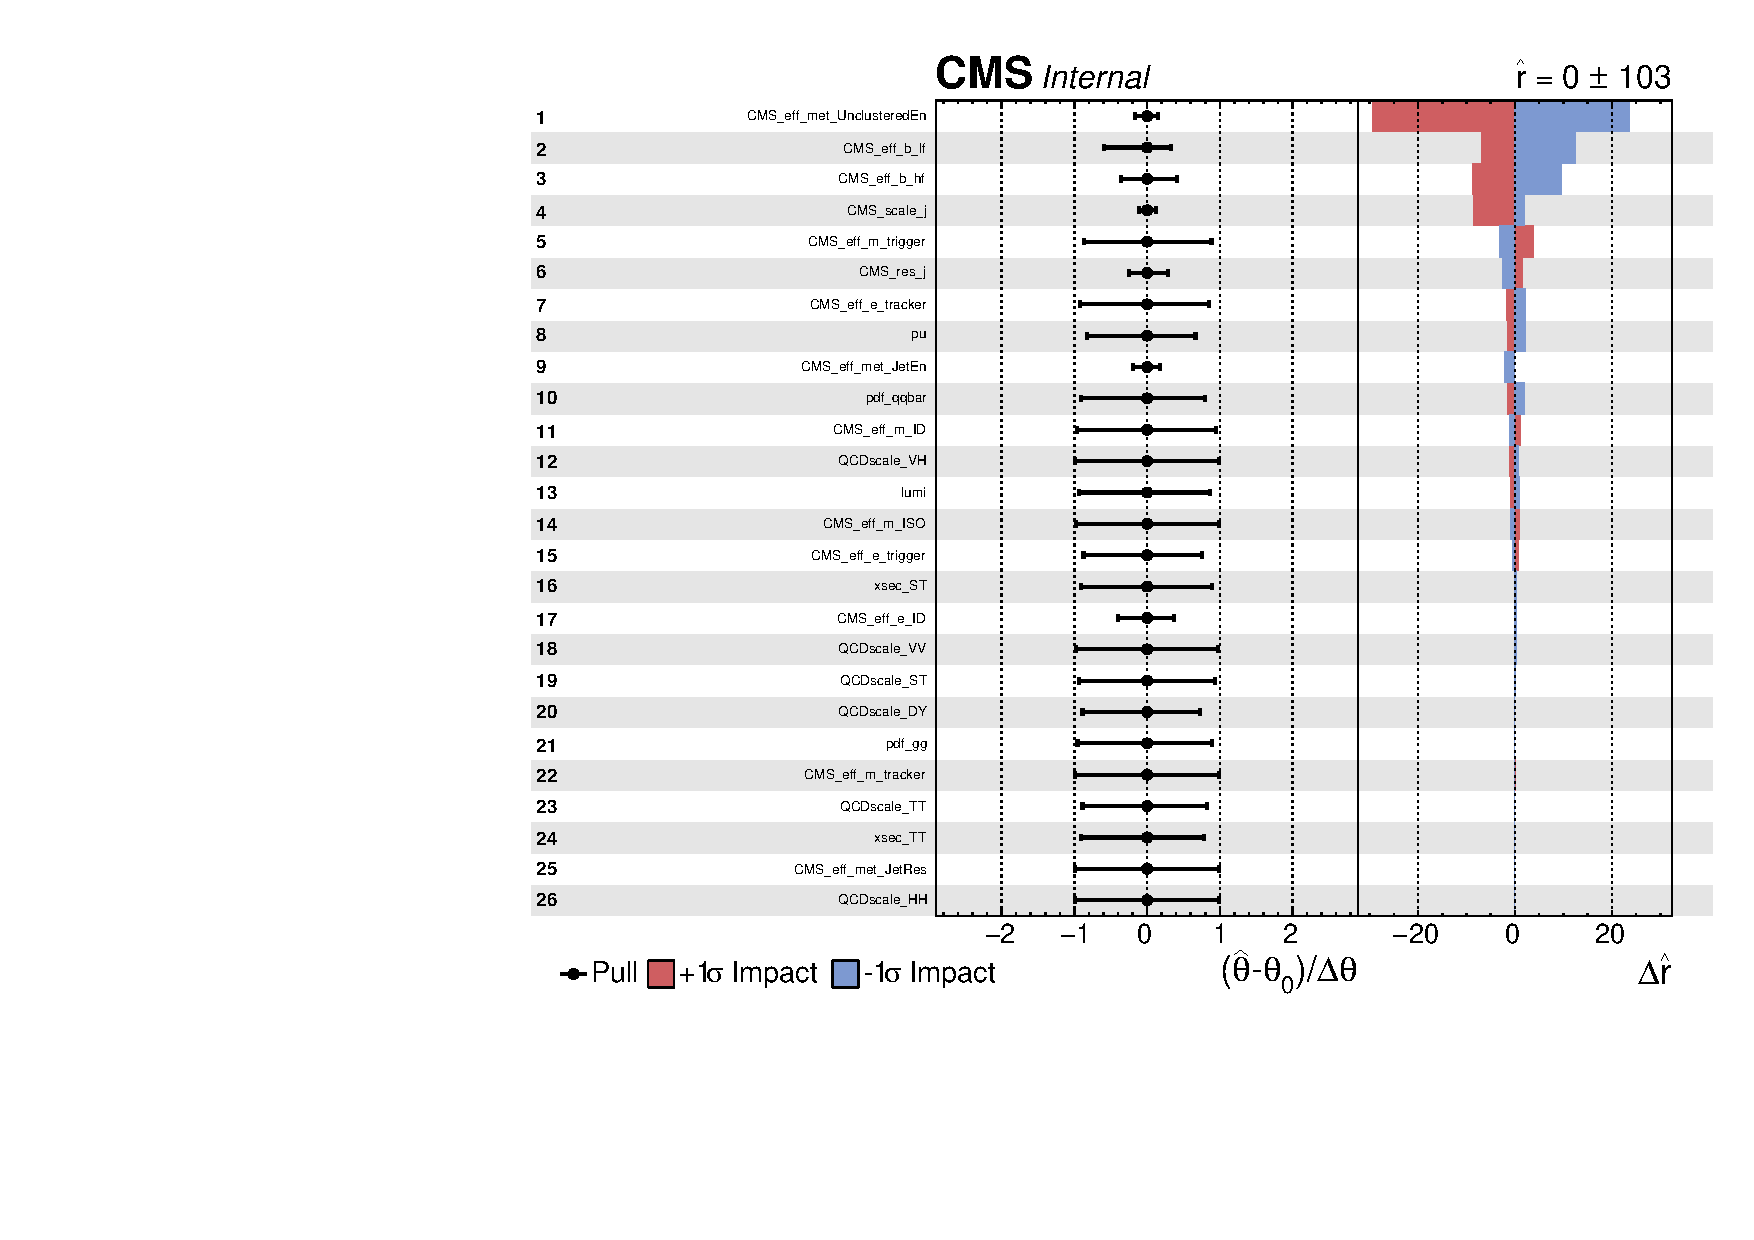
\includegraphics[width=0.5\textheight]{impacts_nov7_300GeV.pdf}
%% %\caption{ Impacts plot for 300 GeV case. Actual limit at this mass point is $248.25_{-71.07}^{+103.9}$~pb.}
%% %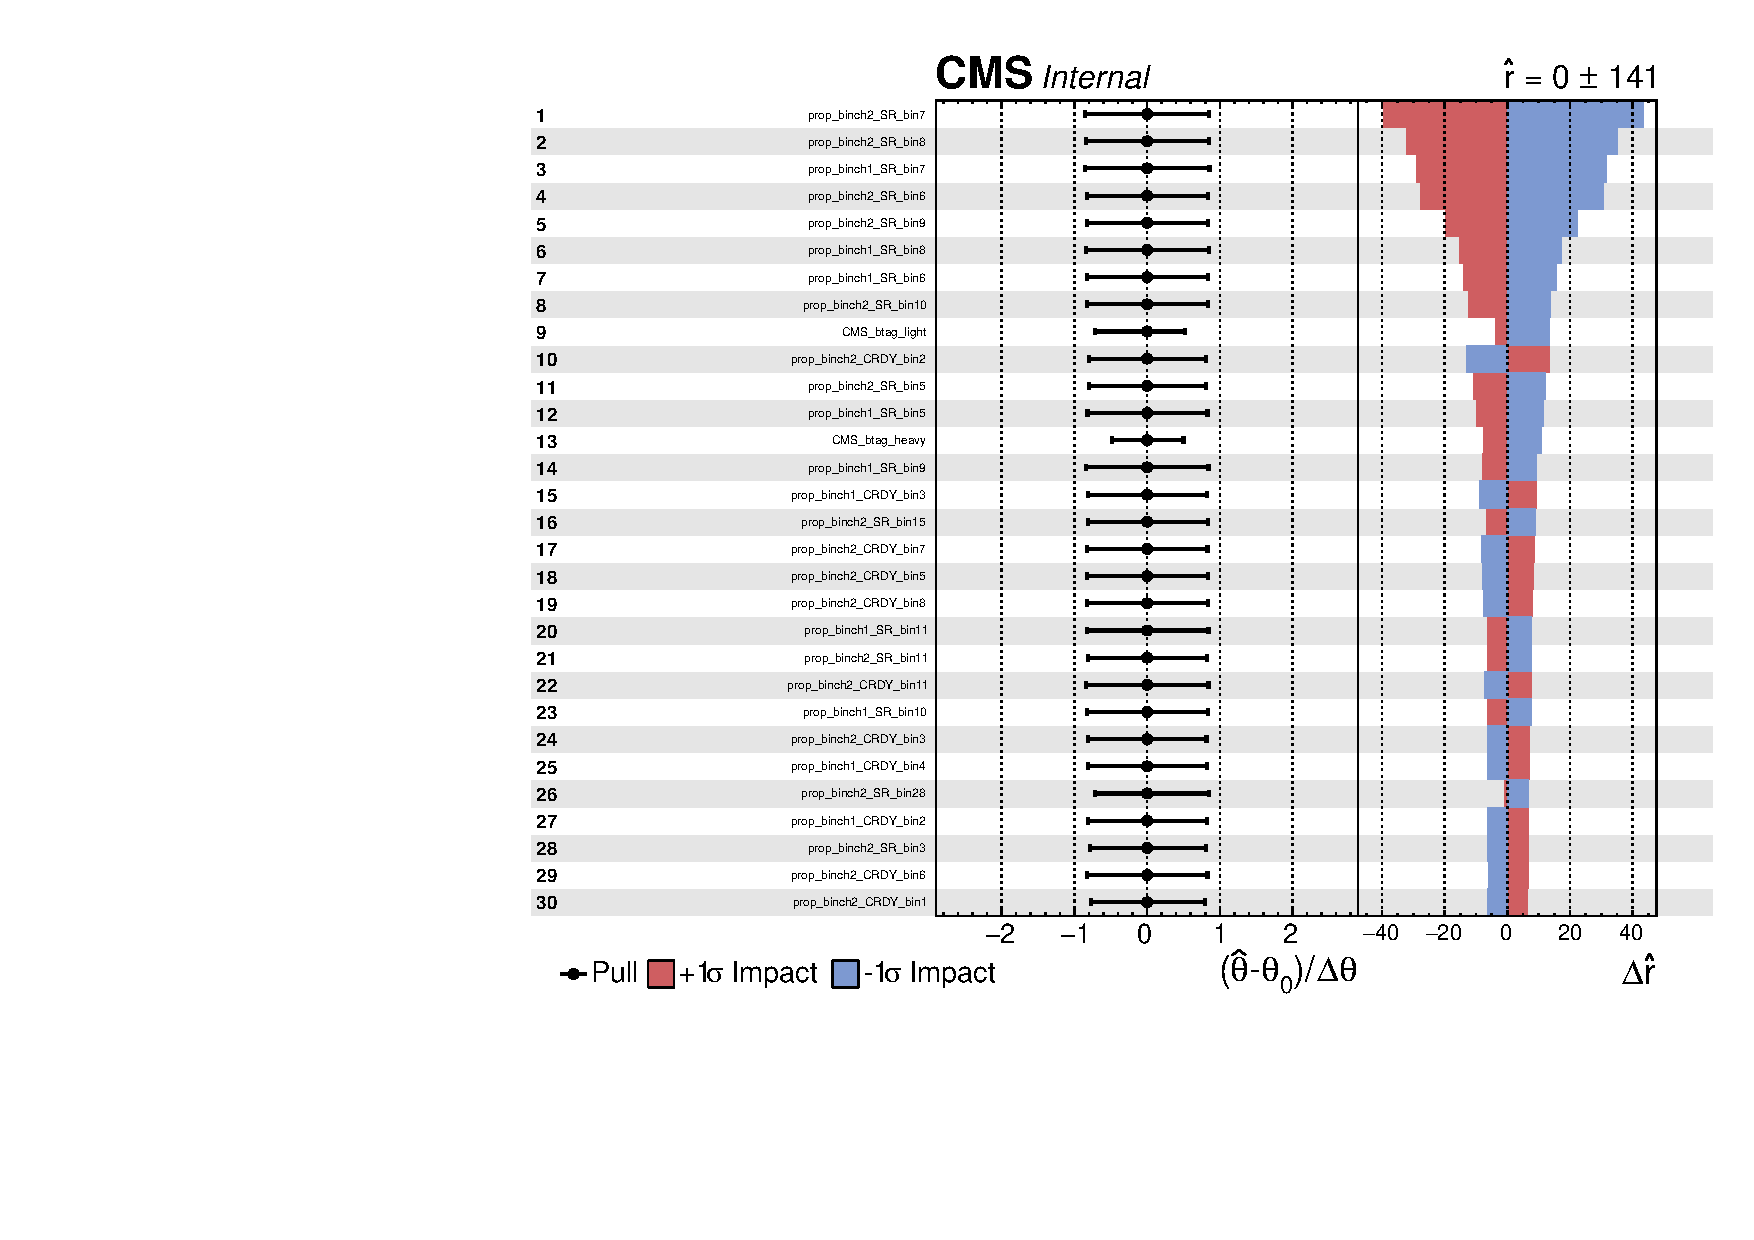
\includegraphics[width=0.5\textheight]{impacts_april6.pdf}
%% 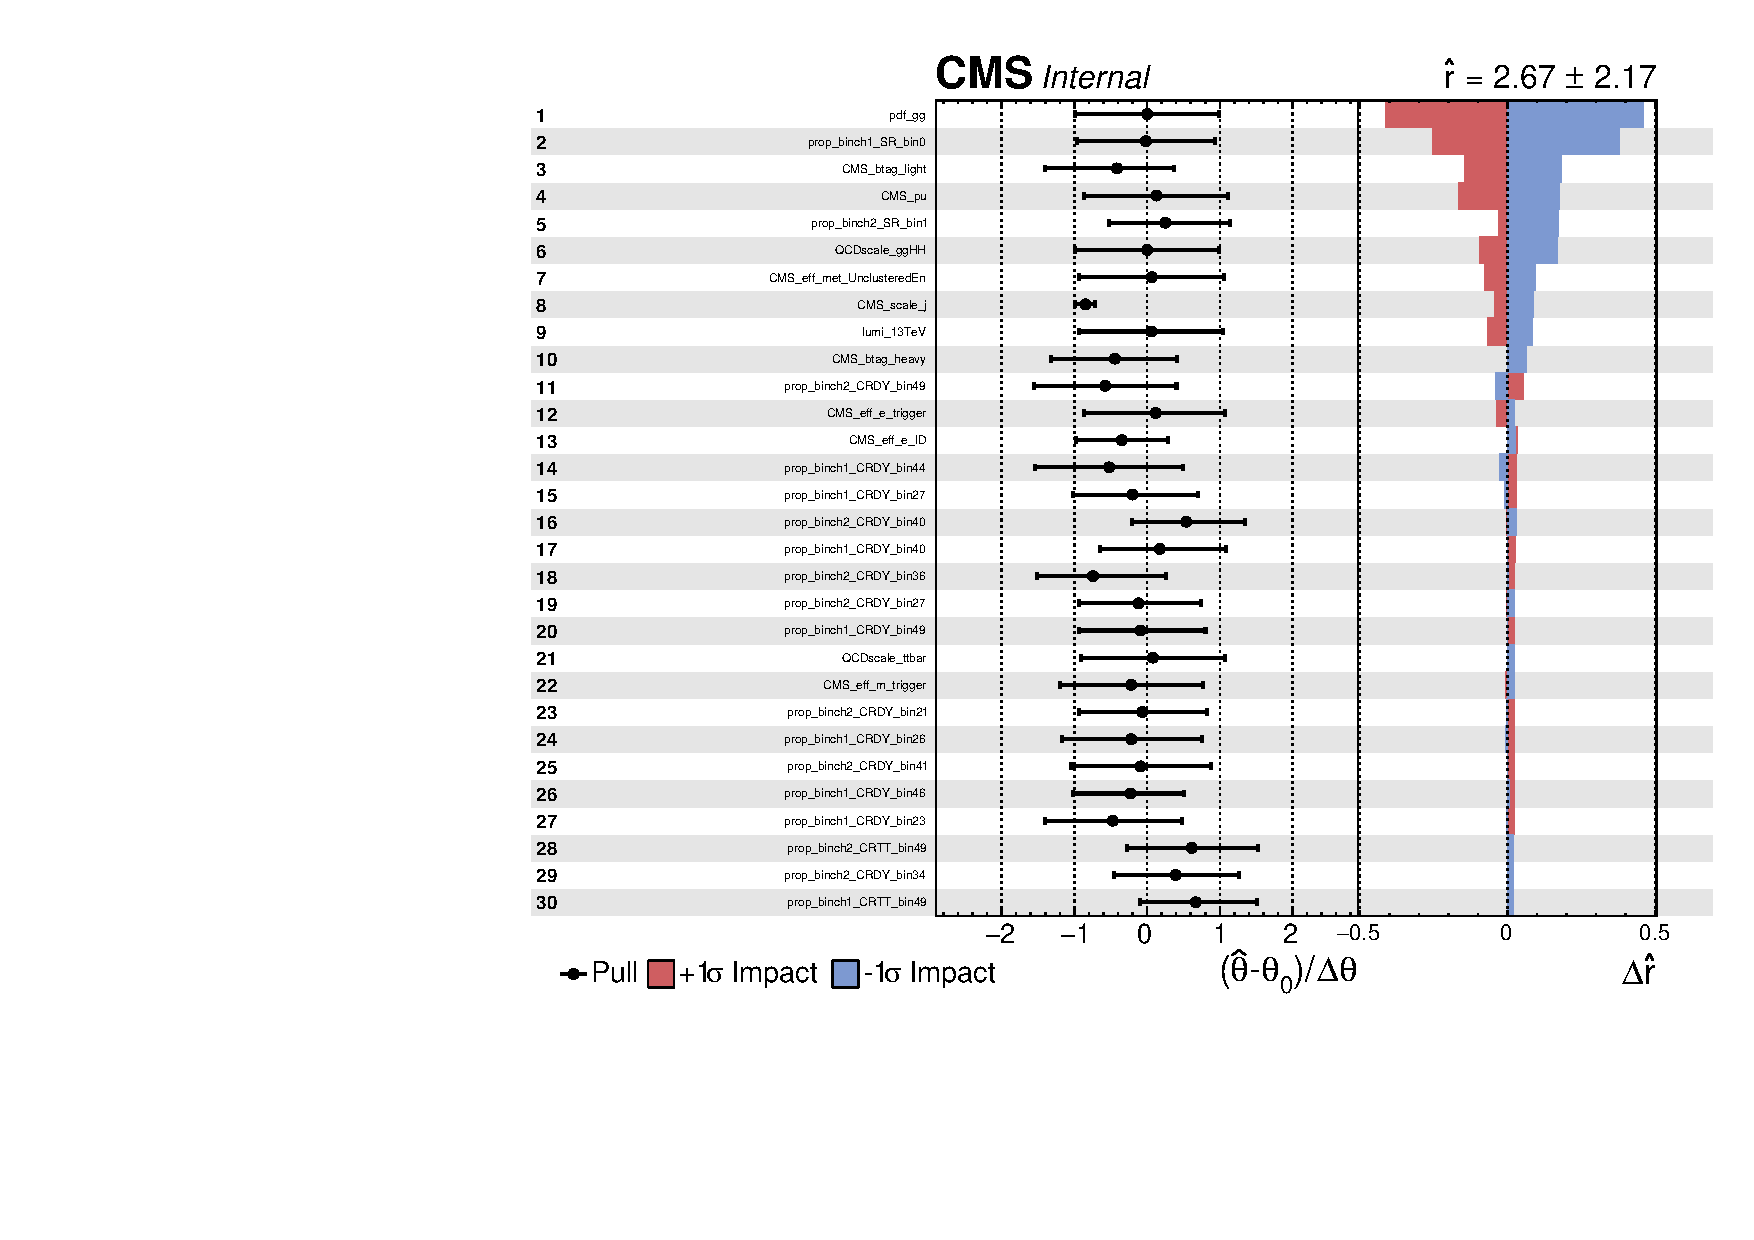
\includegraphics[width=0.5\textheight]{impacts_50_strategy2_july23_300.pdf}
%% 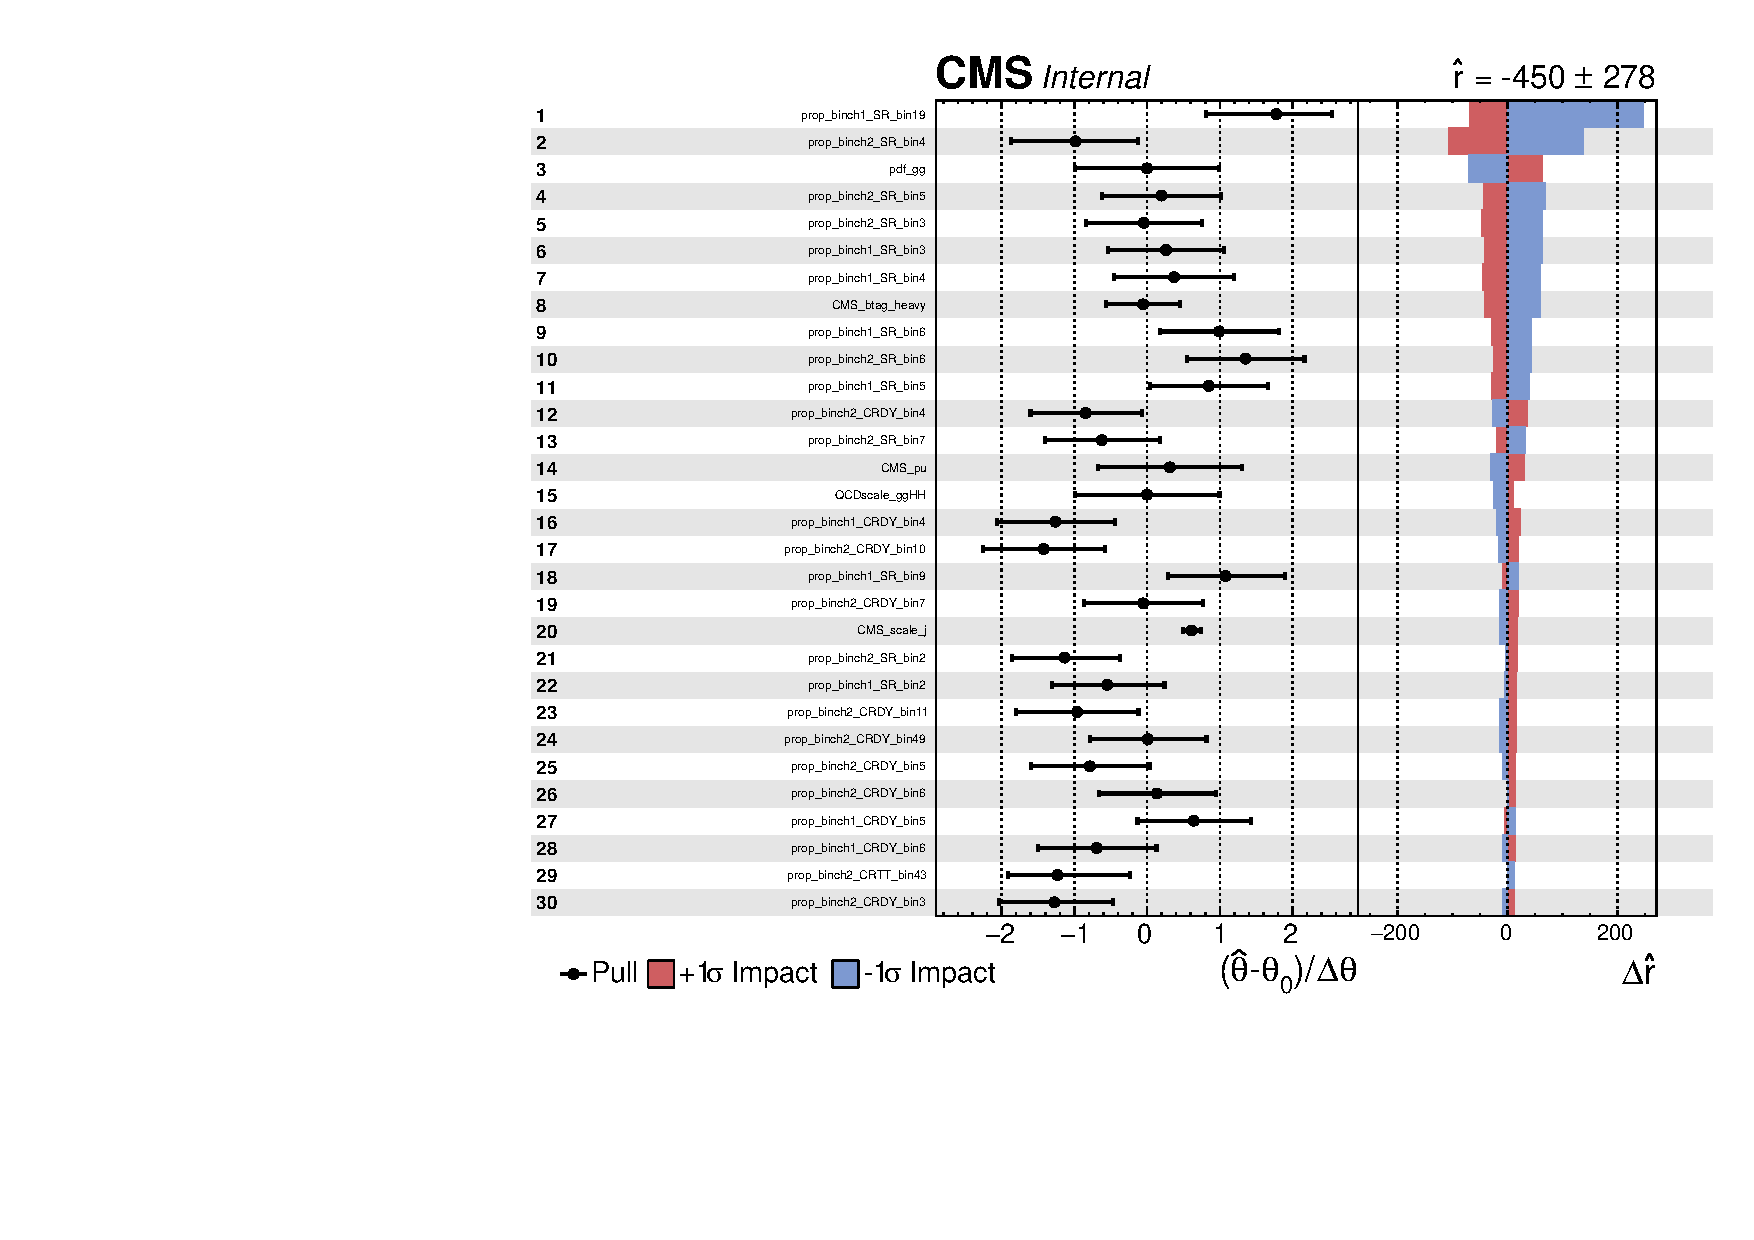
\includegraphics[width=0.5\textheight]{impacts_1500_strategy0_july23_900.pdf}
%% \caption{ Impacts plot for 300(top) and 900 (bottom) GeV case.}% Actual limit at this mass point is $248.25_{-71.07}^{+103.9}$~pb.}
%% \label{fig:impactsBBB}
%% \end{figure}
%% \end{center}



%Following the Higgs PAG list of question for the preapproval checks ~\cite{HiggsPAGPreapprovalChecks}, we produce for 300 GeV case fit results for a background-only Asimov toy (Fig.~\ref{mlfit_Asimov}) and a signal+background Asimov toy (Fig.~\ref{mlfit_Asimov}), with the corresponding outputs of running "diffNuisances.py" that can be found at ~\cite{Comparison_of_nuisances_expectedSignal0_350} and ~\cite{Comparison_of_nuisances_expectedSignal1_350}. 





%\begin{table}


%The impacts plot with BBB uncertainties can be found at Fig.\ref{fig:impactsBBB}.%~\ref{pulls}.





